\chapter{Ayalxrfna sUtarx}

kirx.sha {\rm 1706} riMda {\rm 1783} avadhiyalilxdadx sivxTasxrelxMDfna sherxVSaThx gaNitajacnx Ayalxrfna koDuge gaNita shAsatxrXkekx apAra sumAru {\rm 900} saMshoVdhanA leVKanagaLanunx baredidAdxne. laGu gaNakada sidAdhxMtavanunx samapaRkavAda riVtiyalilx tiLisidAdxne.

$\sqrt{-1}$ eMbudakekx $i$ eMba cihenxyanunx koTuTx adanunx GAtavAgi $e^x$ eMdu modalu upayoVgisi kalapxnA saMKeyxyanunx parxcArakekx taMdavanu.

bahu muKa Gana matutx jAlAkaqtiya bagegx Ayalxrfna sUtarx bahaLa pArxmuKayxvAdudu.

oMdu bahu muKa Ganadalilx $V$ shaqMgagaLanUnx, $F$ muKagaLanUnx matutx $E$ aMcugaLanUnx sUcisidare Aga $V+F=E+2$ Aguvudu eMdu tiLisidavanu 

keVvala {\rm 5} karxma GanAkaqtigaLu sAdhayx avugaLeV
\begin{enumerate}
\item[{\rm 1)}] karxma catuSapxlaka (catumuRKa Gana),
\item[{\rm 2)}] karxmaSaSaThxPalaka (SaNumxKa Gana)
\item[{\rm 3)}] karxma aSaTxPalaka (aSaTx muKa Gana)
\item[{\rm 4)}] karxmadAvxdashaPalaka (dAvxdashamuKa Gana)
\item[{\rm 5)}] karxma viMshatiPalaka (viMshati muKa Gana)
\end{enumerate}

udAharaNege karxma aSaTxPalaka (SaNumxKa Gana)dalilx \quad $v=8$, \quad $F=6$ matutx $E=12$ 
\begin{align*}
\therefore \;\; 8+6 &=12+2\\
14 &=14
\end{align*}

$V+F=E+2$ eMba Ayalxrfna sUtarx meVle tiLisida {\rm 5} karxma GanAkaqtigaLige mAtarx anavxyisutatxde.

bahu PalakagaLalilx avugaLa mUlaka hAdu hoVguva suraMgagaLidadxre I sUtarx anavxyisuvudilalx.

udAharaNege: TeYrinoLagiruva gALi tuMbida TUyxbf iruva hAge
\begin{figure}[H]
\centering
\includegraphics{src/figures/m-147.eps}
\end{figure}

oMdu jAlA kaqtiyalilx $N$ saMpAta biMdugaLa {\rm (node)} saMKeyx, $A$ kaMsagaLa saMKeyx matutx $R$ samatalavanunx valayagaLanAnxgi viBAgisuva saMKeyxyAgidAdxga.

$N+R=A+2$ eMdu tiLisidAdxne udAharaNege
\begin{figure}[H]
\begin{minipage}[c]{4cm}
\centering
\includegraphics{src/figures/m_149.eps}
\end{minipage}
\qquad\qquad 
\begin{minipage}[c]{4cm}
\begin{gather*}
N = 5, \; R=5, \; A = 8, \\
5+5 = 8+2\\
10 = 10
\end{gather*}
\end{minipage}
\end{figure}

koVnisf bagfRna ELu seVtuvegaLa samaseyxge parihAra niVDiruvudu Ayalxrfna hesarinalilx parxKAyxtiyAgide.

aSeTxV alalx Ayalxlarfna ELu seVtuveya samaseyxya vishelxVSaNeyu gaNita shAsatxrXda nUtana vidhAnavAda ToVpoVlajige nAMdiyAyitu.

{\rm 1783} ralilx liyonADoR Ayalxrf mAyAcwkagaLa racaneyalilx toDagidAdxga sUDoku anunx shoVdhisida eMdu tiLidu baMdide.

